\documentclass[prl,aps,twocolumn,floatfix,amsmath,amssymb,superscriptaddress,tightenlines]{revtex4}
\usepackage{graphicx}% Include figure files
\usepackage{epstopdf}
%\usepackage{amsmath}
\usepackage{amsfonts}
\usepackage{bm}
%\bibliographystyle{prsty}
\begin{document}

\date{\today}
\title{Valence Bond and von Neumann Entanglement Entropy in Heisenberg Ladders}
\author{Ann B. Kallin}
\affiliation{Department of Physics and Astronomy, University of Waterloo, Ontario, N2L 3G1, Canada} 

\author{Iv\'an Gonz\'alez}
\affiliation{Centro de Supercomputaci\'on de Galicia, Avda.~de~Vigo~s/n, E-15705 Santiago de Compostela, Spain}

\author{Matthew B. Hastings}
\affiliation{Microsoft Research, Station Q, CNSI Building, University of California, Santa Barbara, CA, 93106}

\author{Roger G. Melko}
\affiliation{Department of Physics and Astronomy, University of Waterloo, Ontario, N2L 3G1, Canada} 

\begin{abstract} We present a direct comparison of the recently-proposed
valence bond entanglement entropy and the von Neumann entanglement entropy on
spin 1/2 Heisenberg systems using quantum Monte Carlo and density-matrix
renormalization group simulations.  For one-dimensional chains we
show that the valence bond entropy can be either less or greater than the
von Neumann entropy, hence it cannot provide a bound on the latter.  On
ladder geometries we reproduce a multiplicative logarithmic correction
previously found in the area law for the valence bond entropy in the
two-dimensional limit.  In contrast, in the N\'eel state the von Neumann entropy
obeys the area law without correction.

\end{abstract}
\maketitle

%\newpage

{\it Introduction.}-- Entanglement has arisen 
as a new paradigm for the study of correlations in condensed matter systems.  
Measurements
of entanglement between subregions, chiefly using entropic
quantities, have an advantage over traditional two-point correlation
functions in that they encode the total amount of information shared
between the subregions without the possibility of missing ``hidden''
correlations \cite{wolf}.  
Such correlations may occur in some quantum groundstates,  for example spin liquid states, 
where two-point correlation functions decay at large lengthscales, however a type of topological order can exist that is quantified in a ``topological entanglement
entropy''  \cite{ KP}.
This and other entropic measures are typically discussed in the context of
the von Neumann entanglement entropy ($S^{\rm vN}$), which for a system partitioned into
two regions A and B, quantifies the amount of entanglement of A with B as
\begin{equation} 
S^{\rm vN}_A = - {\rm Tr} [ \rho_A \ln \rho_A ]. \label{vNEE} 
\end{equation}
Here, the reduced density matrix $\rho_A = {\rm Tr}_B | \psi \rangle
\langle \psi |$ is obtained by tracing out the degrees of freedom
associated with the region B.

The properties of $S^{ \rm vN}$ are well-studied in the field of quantum information theory.
In interacting one dimensional (1D) quantum systems, exact analytical results are known from conformal
field theories (CFT); they show that, away from special critical points,
$S^{ \rm vN}_A$ scales as the size of the boundary between A and B.
This so-called {\it area law} \cite{Shredder} is also believed to hold in many
groundstates of two dimensional (2D) interacting quantum systems,
although few exact results are available \cite{ALreview}.  This has 
consequence in the
rapidly-advancing field of computational quantum-many body theory, where
it is known for example that groundstates of 1D Hamiltonians that satisfy an area law
can be accurately represented by Matrix Product States (MPS) \cite{MPS_DMRG}.
Tensor-network extension of MPS states form a promising new class of numerical algorithms \cite{PEPS1} 
that may allow simulations of 2D quantum systems not amenable to quantum Monte Carlo (QMC) due to
the notorious sign problem.  However, tensor network states
are constructed to obey an area law; in order to be represented faithfully
by them, a given 2D quantum groundstate must have physical entanglement
properties which also obey the area law \cite{ALreview}.

%However, it is believed that 2D
%states which lend themselves to accurate approximation by such methods
%must also obey an area law.

%\begin{figure} { 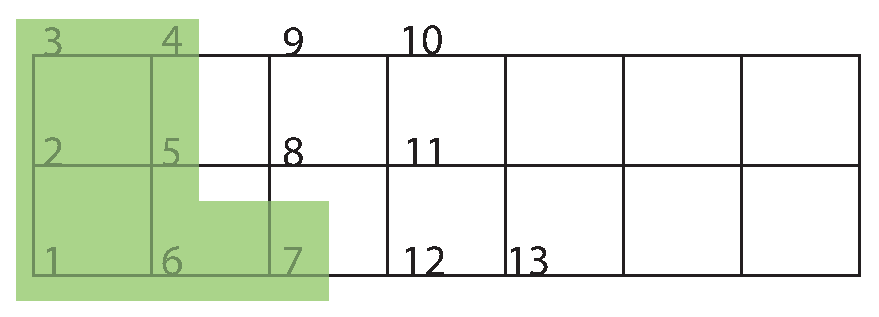
\includegraphics[width=2.4in]{ladder.eps}
%\caption{(color online) A three-leg ladder.  The site labels $x$ indicate
%the order in which DMRG sweeping takes place, which is also the index
%order by which entanglement entropy is measured.  The blue box labels
%sites in the region A, with $x=7$.  \label{ladder}}} \end{figure}

Unfortunately, entanglement is a difficult quantity to
measure in 2D systems, due to the fact that QMC 
%- currently the only scalable method capable of unbiased 2D simulations - 
does not have
direct access to the groundstate wavefunction $| \psi \rangle$, required
in Eq.~\eqref{vNEE}.  In response to this, several authors \cite{Alet,
Chh} have introduced the concept of {\it valence bond} (VB)
entanglement entropy ($S^{\rm VB}$), defined for a  spin system as
\begin{equation} 
S^{\rm VB}_A = \ln(2) \cdot \mathcal{N}_A, \label{VBEE}
\end{equation} 
where $ \mathcal{N}_A$ is the number of singlets
${( |\uparrow \downarrow \rangle - | \downarrow \uparrow
\rangle)/\sqrt{2}}$ crossing the boundary between regions A and B.  Unlike
the $S^{ \rm vN}$, $S^{\rm VB}$ can be accessed easily in the valence-bond basis
projector QMC method recently proposed by Sandvik \cite{Sandvik}.  As
demonstrated in Refs.~\cite{Alet,Chh}, $S^{\rm VB}$ has many properties in
common with $S^{ \rm vN}$, in particular the relationship $S_A = S_B$, and the
fact that $S^{VB}_A=0$ for regions ``un-entangled'' by valence bonds.
A comparison of the scaling of $S^{\rm VB}$ for (critical) 1D spin
1/2 Heisenberg chains shows good agreement with analytical results known
from CFT, however in the
 2D isotropic Heisenberg model it
displays a {\it multiplicative} logarithmic correction to the area law \cite{Alet,Chh}.  If
true also for the $S^{ \rm vN}$, this fact would have negative consequences for the simulation of the 
N\'eel groundstate using tensor-network simulations.

%If this
%property were to be shared by the VN EE, it could have the consequence
%that the 2D N\'eel groundstate can not be approximated by a tensor-network,
%and is therefore not amenable to simulation techniques based on the MPS
%framework
 
In this paper, we compare $S^{\rm VB}$ calculated by valence-bond QMC to 
$S^{ \rm vN}$ accessible through density-matrix renormalization group
(DMRG) simulations of the Heisenberg model on $N$-leg ladders.    For $N=1$, the CFT central charge calculated  by scaling
$S^{ \rm vN}$ shows excellent agreement to $c=1$, whereas $S^{\rm VB}$ converges
to $c<1$.
For $N>1$, $S^{\rm VB}$ is systematically greater than $S^{ \rm vN}$,
a trend which grows rapidly with $N$. An
examination of entanglement defined by bisecting multi-leg ladders
shows a logarithmic correction for the valence-bond entanglement entropy, $S^{\rm VB}_A /N = N \ln
N$ (in agreement with Refs.~\cite{Alet,Chh}), however for data up to
$N=6$, the von Neumann entanglement entropy  convincingly shows a scaling of
$S^{\rm vN}_A /N = N$, thus obeying the area law.



{\it Model and Methods.}-- We consider the spin 1/2 Heisenberg
Hamiltonian, given by  $H =  \sum_{\langle i j \rangle} {\mathbf S}_i
\cdot {\mathbf S}_j \label{ham}$, where the sum is over nearest-neighbor
sites.  Geometries studied are 1D chains, and multi-leg ladders with
length $L$ and number of legs $N$.  
%Many properties of this model on open-boundary ladders with $n$ legs has
%been exhaustively studied.  Of importance, it is known that a spin gap
%exists for even-$n$ ladders in the limit of $L\rightarrow \infty$,
%whereas odd-$n$ ladders behave somewhat more like quasi-1D  systems with
%spin $n/2$ and, from Haldane's conjecture, are therefore gapless.  
We employ two complementary numerical techniques, the valence-bond basis QMC and DMRG, both of
which give {\it unbiased} approximations to the ground state of the
Hamiltonian at zero temperature.  $S^{ \rm vN}_A$ is naturally accessible
through the DRMG 
% I don't think we need this,
%``sweeping'' 
algorithm~\cite{White92}.  At each
step of the algorithm, the wavefunction of the system is approximated by
keeping only the states with largest coefficients in the Schmidt
decomposition for a given bipartition into regions A and
B~$\equiv\complement$A. To find the
basis entering the Schmidt decomposition for region A, the reduced
density matrix $\rho_A$ is calculated and diagonalized, thus allowing easy
calculation of Eq.~\eqref{vNEE}. The truncation of the basis implies that
only a lower bound for $S^{\rm vN}_A$ is calculated, so care must be taken
to ensure that enough of the eigenvalue spectrum is included to converge
$S^{ \rm vN}_A$ to sufficient accuracy; typically the number of states required
is larger than that needed to converge the energy alone.

$S^{\rm VB}_A$ \cite{Alet,Chh} can be calculated using the valence-bond basis
QMC proposed by Sandvik \cite{Sandvik}.  The 
algorithm that we use is the simple single-projector method, with lattice
geometries constructed to match those used by the DMRG algorithm.  The
ground state of the system is projected out by repeated application of a
list of bond operators on nearest neighbor sites of the ladder.  A number
of bond operators are changed each step and the change is accepted
with a probability depending on the number of nearest neighbor bonds in
the resulting valence bond states. Measured quantities such as energy or
$S^{\rm VB}_A$ are then calculated by a weighted average over all the valence bond
states obtained by this procedure.

\begin{figure} {
%\includegraphics[width=3.2in]{fig1_inset.eps}
\includegraphics[width=3.3in]{4-panelFIG1.eps} \caption{(color online) Valence-bond
and von Neumann entanglement entropies for a 1D Heisenberg chain with PBC and OBC. Upper panels show the entropies as a
function of the conformal distance $x'$ for 100-site chains (see text).
Lower plots show the values for the central charge $c$, obtained by
fitting the numerical data to the CFT result, for several chain lengths.
For PBC, $c$ is calculated with the two smallest $x'$ points removed.
For OBC, the fits depend on the number of sites included in the fit, $z$,
which we
%To bypass these effects we plot $c$ as
%a function $z$ for each $L$. Here, $z$ is 
systematically decreased by
removing $x'$ data points from the {\it outside} ends of the chain.
$c$ is illustrated for $S^{\rm vN}$ (closed symbols) and $S^{\rm VB}$ (open
symbols) for system sizes $L=64$ (circles), $L=100$ (squares), $L=128$
(diamonds), and $L=200$ (triangles) \label{1D}}} \end{figure}

{\it One-dimensional chain.}-- We consider first the case of Heisenberg
chains ($N=1$). We employ both open (OBC) and periodic (PBC) boundary conditions
with our DMRG and QMC simulations, noting that in DMRG, PBCs typically
have poorer convergence properties than OBCs and more states must be kept
in each truncation.  The DMRG algorithm requires each region A and B to
be topologically connected, so in 1D the bipartition is defined by a site
index $x$ with sites within the interval $[1,x]$ ($[x+1,L]$) belonging to
region $A$ ($B$), $L$ being the length of the chain.  From the
remainder of this paper, we label $S_A$ by its site index, $S(x)$.
We stress that the QMC and DMRG results are on the same geometry and
Hamiltonian, and reproduce the same ground state energies; Figure 1 and subsequent figures can be considered as exact comparisons between the $S^{\rm VB}_A$ and $S^{ \rm vN}_A$.

The 1D Heisenberg model is known to be critical and therefore can be
mapped to a 2D classical Hamiltonian at its critical point, which
can be described by CFT in the limit $L\to\infty$.  To address
finite-length chains one can use the conformal mappings $x\to x'=L/\pi
\sin(\pi x / L)$ for PBC, and 
%$x\to x'=2L/\pi \sin(\pi x / L)$ 
$x\to 2x'$ for OBC. %VN EE 
Calculations within CFT~\cite{Cardy} obey $S^{\rm vN}(x)= c/3
\ln(x') + S_1$ in the PBC case, and $S^{\rm vN}(x)= c/6 \ln(2x') +
\ln(g)+S_1/2$ in the OBC case, where $c$ is the central charge of the CFT,
$S_1$ is a model-dependent constant, and $g$ is Ludwig and Affleck's
universal boundary term~\cite{AffleckAndLudwig}.

Figure~\ref{1D} illustrates simulation results in both cases, the left
(right) panels corresponding to PBC (OBC). 
%In Refs.~\cite{Alet, Chh}, VB
%EE calculated from QMC was compared to the CFT result, and a good fit to a
%central charge of $c=1$ was found for both cases.  In Fig.~\ref{1D} we
%compare this result to the VN EE calculated from the DMRG.  
For PBC both
$S^{\rm VB}$ and $S^{ \rm vN}$ are seen to fit well to the CFT result, although
$S^{ \rm vN} > S^{\rm VB}$. The regression fit shows very good
convergence with the central charge predicted by CFT, $c=1$, for $S^{ \rm vN}$, while
$S^{\rm VB}$ fit yields a lower value than predicted.
{\bf ANN: ADD DISCUSSION OF UNIVERSAL g (?)}.  
%TODO {\it (Should I include this?) It is possible the VB EE data is not
%sufficiently converged which would could give results below the CFT
%predicted value, however data from Refs.~\cite{Alet,Chh} bears similar
%results. }

For OBC both $S^{ \rm vN}$ and $S^{\rm VB}$ split into two branches, the upper (lower)
corresponding to an odd (even) number of lattice sites in $A$.  This
reflects a well-known ``dimerization'' effect induced by OBC~\cite{Ian1}.
Notice that contrary to the PBC case, $S^{ \rm vN}$ is now \textit{smaller}
than $S^{\rm VB}$. A regression fit of the lower branch to the form $c/6 \ln
({2x'})$ (inset) shows excellent convergence of $S^{ \rm vN}$ to the central
charge predicted by CFT, $c=1$, once finite-size effects and the proximity
of the data to the open boundaries are taken into account.  In contrast,
$S^{\rm VB}$ fit deviates significantly from the CFT result for larger system
sizes, give $c>1$ when all or most data is included in the fit, and $c<1$
as data is systematically excluded from the fit (data closest to the open
boundary is removed first).

{\it Multi-leg ladders.}-- Moving away from the 1D chain, one can add
``legs'' to the lattice in a systematic way. In this case the sum over
nearest neighbors is extended to neighbors along rungs as well as along
legs.  As it was noted before, DMRG imposes contraints to the subregion
geometry. In multi-leg ladders we choose to move in a 1D path that visits
first bonds sitting in rungs rather than bonds sitting in legs (see
Fig.~\ref{ladder}).  DMRG computational demands increase dramatically with
the number of legs, so in this paper we restrict ourselves to ladders with
OBC up to $N=6$ legs. QMC lacks this limitation and one can go up to
$N=20$ with minimal CPU effort.

\begin{figure} { \includegraphics[width=3.3in]{FIG23NEW.eps}
\caption{(color online) Entanglement entropies for 3-leg (left)
and 4-leg (right) ladder systems with OBC and 100 sites per leg.  For
(gapless) odd-leg ladders, $S(x)\propto\ln(x')$.  The left
inset shows $S(x)$ as a function of the conformal distance, $x'$, on a log
scale. For (gapped) even-leg ladders, $S(x\gtrsim\xi)=const.$
%For odd-leg ladders (gapless) $S(x)$ is convex with a maximum at $x=L/2$.
%Left inset shows $S(x)$ as a function of the conformal distance, $x'$, on
%a log scale, satisfying $S(x)\propto\ln(x')$. For even-leg ladders
%(gapped) $S(x\gtrsim\xi)=const.$ Both cases show the branched structure
%discussed in the text. 
The right inset shows the site indexing used for multi-leg ladders with the
bipartition for $x=9$.  \label{ladder} }} \end{figure}

Figure~\ref{ladder} shows $S^{ \rm vN}$ and $S^{\rm VB}$ calculated
for the 3-leg and 4-leg ladder. As happens with the OBC 1D chain, $S^{\rm VB} > S^{ \rm vN}$ .  
The entropies show different behavior depending on
$N$ being even or odd.  Even-leg ladders are known to have a
spin-gap~\cite{White1994}, and therefore only sites within distances from
the boundary between A and B {\it smaller} than the correlation length
$\xi$ contribute to the entanglement, yielding $S(x\gtrsim \xi)= {\rm
const}.$ In contrast, odd-leg ladders are gapless, and therefore all the
sites within regions A and B contribute to the entanglement, 
%yielding a convex $S(x)$ with a maximum at $x=L/2$, 
yielding $S(x)\propto\ln(x')$, 
which follows the CFT result in
analogy to the 1D case. As can be seen $S(x)$ splits in branches, with a
(quasi-)periodic structure superimposed to the main dependence on $x$,
the period being $N$ ($2N$) for even- (odd-)leg ladders. This reflects the
periodicity of the underlying 1D path in which we move, and the fact that
valence bonds within the same rung are energetically
favored~\cite{White1994}. The doubling of the period for odd-leg ladders
is due to the same dimerization effect as in Ref.~\cite{Ian1}.

%%A qualitative explanation based on a RVB picture is the
%%following~\cite{White1994}. In ladder geometries, short-range singlets
%%between sites in the same rung are favored, as can then resonate to
%%``plaquette'' configurations. This causes the branched structure with
%%period $N$. Singlets between distant sites freeze the VB configuration in
%%region they cross, preventing this resonance and increasing the energy of
%%the system.  Even-leg ladders can be fully covered by ``in-rung''
%%singlets, and have strongly entangled rungs weakly entangled among them.
%%On the contrary, odd-leg ladders can not be fully covered by ``in-rung''
%%singlets, leaving one ``un-paired'' site per rung, which can entangle
%%distant sites without penalty in energy, similarly to the 1D case. The
%%doubling of the period for odd-leg ladders is due to the same dimerization
%%effect as in Ref.~\cite{Ian1}.
 
{\it Area law in multi-leg ladders.}--  
We can use these multi-leg ladder results to address the question of the adherence of the 2D N\'eel state
to an area law.  To do so, we
define the lattice
geometry such that region A is rectangular, cutting a multi-leg ladder
cleanly across a rung, such that the ``area'' separating region A and B is
equivalent to the number of legs in the ladder $N$.  We chose this area A
to contain contain $2N^2$ sites to have an aspect ratio of order unity; in
contrast, the entanglement entropy of a long
skinny region would be dominated by the behavior
of the single gapless mode for odd-leg ladders.

Figure~\ref{zigzag} illustrates the simulation results for $N$-leg ladders.
Plotting $S/N$ versus $N$ on a log scale, one sees that we obtain a
multiplicative logarithmic correction to the $S^{\rm VB}$ area law, in agreement
with results from Refs.~\cite{Alet,Chh}.  However, the linear slope is {\it not} present in
the plot of the $S^{ \rm vN}$ data from the DMRG, which convincingly approaches a
constant for large $N$.  Clearly, for $S^{ \rm vN}$ the area law is
indeed obeyed in the N\'eel groundstate, leading one to conclude that the
multiplicative logarithmic correction occurs in $S^{\rm VB}$ only.  We
also present data for free fermions, showing the logarithmic correction to the area law
for $S^{ \rm vN}_{\rm ff}$ in this case\cite{2dfermion}.
In the next section, we explain this 
in the context of the bond length distribution in the QMC.
Contrary to the suggestion in Ref.~\cite{Alet}, a gapless Goldstone mode will {\it not} give a logarithmic
divergence to $S^{ \rm vN}$ since a gapless bosonic mode in 2D
obeys an area law\cite{2dboson}.  We have done a spin-wave calculation of
the entropy for this system and found an area law, albeit with
$S/N\approx 0.2$, slightly lower than suggested for spin~$1/2$ in Fig.~\ref{zigzag}.

%Despite the importance of adherence to the area law in tensor-network
%generalization of MPS techniques, it is still not yet known whether the
%2D isotropic Heisenberg ground state does obey the area law.  The results
%from Refs.~\cite{Alet,Chh} for the VB EE in 2D indicate a multiplicative
%logarithmic corrections to the area law.  We find it necessary to address
%whether the same logarithmic correction exists in the VN EE.
%Fig.~\ref{zigzag} shows the VB EE and VN EE for ladders with N legs.  The
%lattice geometry is chosen such that subregion A contains $2N^2$ sites
%and is always rectangular.  It is clear that Fig.~\ref{zigzag} shows a
%logarithmic correction to the area law for VB EE, in agreement with
%Refs.~\cite{Alet,Chh}.  However, in the case of the VN EE, the data
%approaches a constant value and shows no correction to the area law.

\begin{figure} { 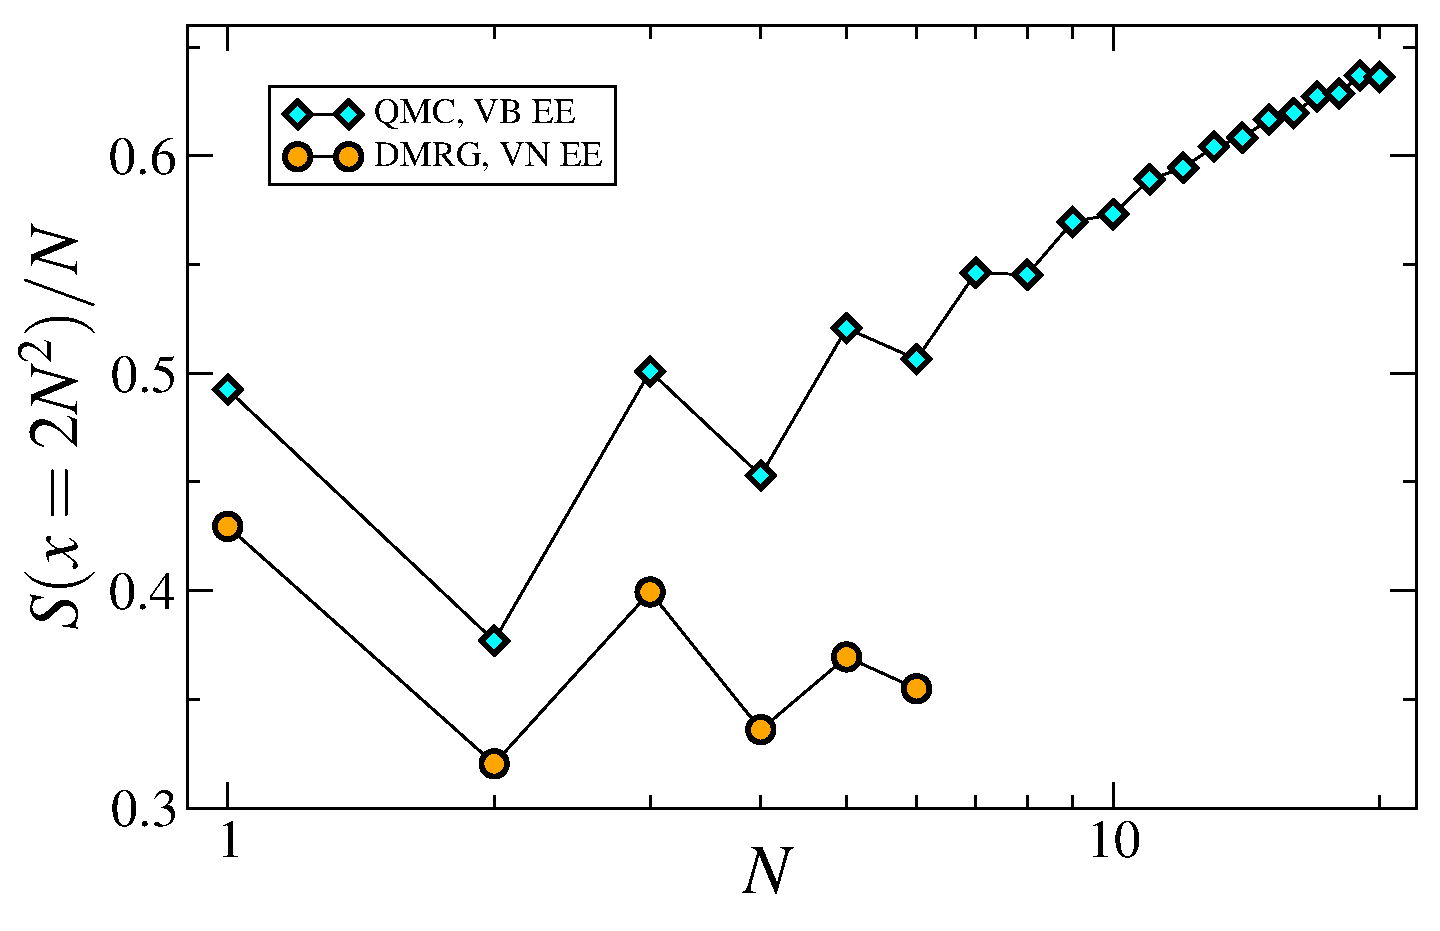
\includegraphics[width=3in]{fig4.eps} \caption{(color
online) Entanglement entropies divided by $N$,  for $N$-leg Heisenberg (filed symbols) and free-fermion (open symbols) ladders, taken such that the region A includes $2N^2$ sites.
%normalized by N, the number of legs.  
All ladders
have 100 sites per leg.  \label{zigzag}}} \end{figure}

{\it Bond Length Distribution---} Sandvik defined the bond length
distribution $P(x,y)$ as the probability of a bond going from site $x$ to
site $y$, and found that $P(x,y)\sim |x-y|^{-p}$ with $p\approx 3$.  
%This value of $p$ gives the logarithmic divergence in the VB EE, as can
%be found by directly calculating the VB EE from $\sum_{x\in A,y\in B}
%P(x,y) \log(2)$.
This value of $p$ gives the logarithmic divergence in $S^{\rm VB}$, as can be
found by directly calculating $S^{\rm VB}_{A}=\sum_{x\in A,y\in B} P(x,y)
\log(2)$.

We can understand the value of $p$ from a scaling argument similar to that used in \cite{network}.
Consider the number of bonds of length $l$ which leave a region of linear size $l$.  For $p>4$, this
scales to zero, and hence should give a phase with no long-range order (indeed, such a phase should
be topologically ordered).  For $p=4$, this number of bonds is $l$-independent, and corresponds to a critical
system ($p=2$ was observed at critical points in 1d\cite{1dcritical}).
For $p<2$, the bond length distribution is not normalized, and all bonds are long, so that
there should be no short-range order.  $p=3$ represents a state with both long-range
and short-range order; we have a handwaving argument that $p=3$ corresponds to a state
with Goldstone modes, since the correlation function of two spins is given by the
probability that they lie on the same loop, and such a probability can be estimated by
the Green's function of a Levy flight taking steps with a power law distribution with power $3$.



{\it Discussion.}-- In this paper, we have compared scaling properties of
the valence bond entanglement entropy ($S^{\rm VB}$) defined in
Refs.~\cite{Alet,Chh} to the von Neumann entanglement entropy ($S^{ \rm vN}$) in the
spin 1/2 Heisenberg model on 1D and multi-leg ladder geometries, using QMC and DMRG simulations.
%Both entropy measurements were evaluated using large-scale numerical
%simulations; the VN EE with DMRG, which is restricted to 1D or seven-leg
%and less open boundary ladders; and the VB EE with valence-bond basis QMC,
%which is avaliable for any lattice dimension or geometry. 
In 1D, we find
that $S^{\rm VB}$ mimics the behavior of $S^{ \rm vN}$ closely, although 
%using
%the definition of Eq.~\eqref{VBEE}, 
it is less than $S^{ \rm vN}$ for periodic
chains, and greater than $S^{ \rm vN}$ for open chains. In addition, fits to
1D conformal field theory, which are excellent for $S^{ \rm vN}$ calculated
via DMRG, appear to deviate significantly for $S^{\rm VB}$ in the large
chain-size limit, approaching some $c<1$ for both boundary conditions.

On multi-leg ladder systems with open boundaries, $S^{\rm VB}$ is
systematically greater than $S^{ \rm vN}$, a discrepancy which grows as the
number of legs is increased.  Defining the boundary between the two
entangled regions as being bipartitioned by a cut across all legs, we can
evaluate the adherence of the entanglement entropies to the area law.  $S^{ \rm vN}$ obeys the area law in the large-leg limit, whereas $S^{\rm VB}$
 reproduces a multiplicative log correction found in
Refs.~\cite{Alet,Chh} for the N\'eel groundstate of the 2D
model.

The fact  that $S^{\rm VB}$ can be either greater or less than $S^{ \rm vN}$ can be understood through simple
examples.  Consider an 8-site chain, with sites 1 to 4 in region A.  Let
$|(ij)(kl)...\rangle$ denote a state in which sites $i,j$ are in a singlet, sites $k,l$ are in a singlet, and so on.
Then, the state $|(12)(34)(56)(78)\rangle+|(14)(32)(58)(76)\rangle$ has vanishing $S^{\rm VB}$ since
no bonds connect $A$ to $B$, but non-vanishing $S^{ \rm vN}$.  
On the other hand, consider a 4-site chain in
the state $|(12)(34)\rangle+|(14)(32)\rangle$, and let region $A$ contain sites $1$ and $3$.  Then, the $S^{\rm VB}$ is maximal,
equal to $2\log(2)$, while $S^{ \rm vN}$ is smaller.  The second state we have
described is in fact the N\'eel state with no
quantum fluctuations: the equal amplitude superposition of all configurations of bonds going from one sublattice to the other.
Thus, it is not surprising that states with N\'eel order show $S^{\rm VB} > S^{ \rm vN}$.

This work has elucidated the relationship between the valence-bond and von Neumann entanglement entropies.
Although clearly a good measurement of entanglement readily accessible to
numerical simulations in 2D and higher, $S^{\rm VB}$ does not provide a bound
on $S^{ \rm vN}$, unlike other entropic measures such as Renyi entropies.
Other properties of $S^{ \rm vN}$, such as its adherence to an area law, are
reproduced in the groundstates of some gapped systems \cite{Alet,Chh},
however in the case of the N\'eel groundstate of the 2D Heisenberg model,
unphysical multiplicative logarithmic corrections appear in $S^{\rm VB}$,
which are not caused by gapless excitations or algebraically decaying
correlations, but simply by the valence-bond length distribution.
% TODO I guess this is done now.
%({\bf we need to justify this in the text}).  
The presence of this correction must
be taken into account in proposals to use $S^{\rm VB}$ for such important
future tasks such as characterizing topological phases 
%using entanglement
%entropy, 
or studying universality at quantum phase transitions.

{\it Acknowledgements.}-- The authors thank I.~Affleck, J.~Berlinsky,
N.~Bonesteel,
A.~Del~Maestro, A.~Feiguin, L.~Hormozi, and E.~Sorensen for useful
discussions.  This work was made possible by the computing facilities of
SHARCNET and CESGA.  Support for this work was provided by NSERC of
Canada (A.B.K. and R.G.M.) and the NSF under Grant No. NSF PHY05-51164 (I.G., M.B.H. and R.G.M).

\bibliography{VB_biblio}

\end{document}
